\documentclass[a4paper,10pt]{article}
\usepackage[utf8]{inputenc}
\usepackage[spanish]{babel}
\usepackage{amsmath}
\usepackage{amssymb}
\usepackage{graphicx}
\usepackage{hyperref}
\usepackage{fancyhdr}
\usepackage{geometry}
\usepackage{enumitem}
\usepackage{titlesec}
\usepackage{caption}
\usepackage{float}
\usepackage{cite}

% Configuración de la página
\geometry{top=2.5cm,bottom=2.5cm,left=2cm,right=2cm}

% Configuración de encabezado y pie de página
\pagestyle{fancy}
\fancyhf{}
\fancyfoot[C]{}
\fancyhead[C]{}

\renewcommand\spanishtablename{Tabla}


% Configuración del tamaño de los títulos
\titleformat{\section}{\normalfont\fontsize{14}{16}\bfseries}{\thesection.}{1em}{}
\titleformat{\subsection}{\normalfont\fontsize{12}{16}\bfseries}{\thesubsection.}{1em}{}
\titleformat{\subsubsection}{\normalfont\fontsize{11}{16}\bfseries}{\thesubsection.}{1em}{}


% Configuración de figuras y tablas
\captionsetup[table]{labelfont=bf,labelsep=period,justification=centering}
\captionsetup[figure]{labelfont=bf,labelsep=period,justification=centering}




% Añade esto al preámbulo
\usepackage{authblk}
% \renewcommand\Authsep{, }
% \renewcommand\Authands{, }
\renewcommand{\Affilfont}{\fontsize{8}{10}\selectfont\bfseries}
\renewcommand{\Authfont}{\fontsize{12}{10}\selectfont}
\setlength{\parskip}{0.5\baselineskip}%
\setlength\parindent{0pt}
\renewcommand{\headrulewidth}{0pt}
\renewcommand{\footrulewidth}{0pt}

\usepackage{xpatch}

\makeatletter
\xpatchcmd{\@maketitle}
  {\@title}
  {\fontsize{17}{20}\selectfont\bfseries\@title}
  {}{}
\makeatother
% Modifica esta parte para definir los autores, afiliaciones y correos
\title{Título del Artículo}
\author[1]{Nombre Apellido}
\author[2]{Nombre Apellido}
\author[1]{Nombre Apellido}
\affil[1]{Institución, Localidad, País}
\affil[2]{Institución, Localidad, País}
\affil[ ]{mail@servidor.com, mail2@servidor.com}
\date{}


\begin{document}

\maketitle
\thispagestyle{empty} % Para no numerar la primera página

\begin{abstract}
Cada artículo deberá comenzar con un resumen de no más de 200 palabras que deberá ser acompañado por una lista de palabras claves (no más de 5) que se vinculen con el contenido del artículo. Sangría de 2 cm antes del texto y 2 cm después del texto. Sin referencias ni fórmulas. Tipografía Times New Roman 10 pt.     
\end{abstract}
\textbf{\emph{Palabras clave:}} indicar una lista de hasta 5 palabras clave separadas por punto y coma (;). La inicial de cada una debe estar en mayúscula. En caso de palabras clave compuestas, poner inicial mayúscula solamente en el primer término; p. ej., ``Materiales educativos'' . Tipografía Times New Roman 10 pt. 

\section{Introducción}
Los artículos deberán estar escritos en español, en tipografía Times New Roman, con espaciado sencillo, texto justificado y cuerpo de texto a una columna.  

Los párrafos estarán en Times New Roman 10 pt  y  el título de sección en Times New Roman 14 pt.

El título del artículo estará centrado en Times New Roman 18 pt. Debajo del mismo, aparecerán los nombres de los autores (en Times New Roman 12 pt) y las referencias de las instituciones de las que forman parte irán por debajo de ellos, al igual que sus e-mails (en Times New Roman 8 pt).

No deberán tener más de 14 páginas tamaño A4. Las páginas no deberán ser numeradas.

Las referencias a otros documentos deben indicarse con un número entre corchetes por orden de aparición y deberán consignarse al final del artículo. 

Esta sección podrá tener una o más subsecciones tituladas del modo indicado. Las secciones y subsecciones del manuscrito deberán distinguirse claramente siguiendo el estilo presentado en esta plantilla. 

La primera sección del artículo debe ser una introducción que contendrá el análisis general de la problemática y las referencias principales. Se sugiere incluir en la introducción una descripción sintética del aporte del artículo.

La última sección del artículo deben ser las Conclusiones. Puede incluir las líneas de trabajo/investigación a seguir.

\subsection{Título Subsección}
Texto (Times New Roman, 10 pt). Título de subsección (Times New Roman, 12 pt). 


\subsection{Título Subsección}
Texto.

\section{Título Sección}
Se agregarán tantas secciones (con sus subsecciones) como sea necesario.

\subsection{Título Subsección}
Texto.

\subsubsection{Título Subsubsección}

Texto. Título de la subsubsección en 11 pt.

Las \textbf{figuras, tablas y gráficos} se intercalarán en el texto después de su primera mención, indicando su número de orden y título. (Ej: \emph{Figura} \ref{fig:ejemplo}. Título de la figura). 

\begin{figure}[H]
    \centering
    % scale=0.8 shrinks it to 80% of its size; adjust as needed
    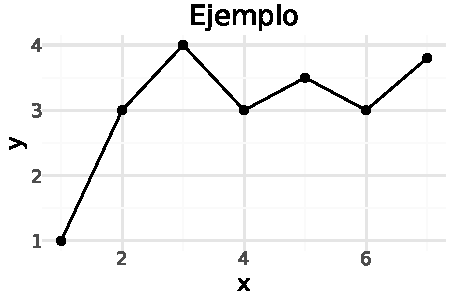
\includegraphics[scale=0.8]{ejemplo.pdf} 
    \caption{Título de la Figura (Datos de ejemplo.pdf)}
    \label{fig:ejemplo}
\end{figure}

En el caso de las tablas (ver \emph{Tabla \ref{tab:ejemplo}}. Tabla de ejemplo), el epígrafe debe colocarse en la parte superior y en las figuras y gráficos al pie. 

\begin{table}[H]
    \centering
    \caption{Título de la Tabla de ejemplo}
    \begin{tabular}{|c|c|c|}
        \hline
        Columna 1 & Columna 2 & Columna 3 \\
        \hline
        Dato 1 & Dato 2 & Dato 3 \\
        \hline
    \end{tabular}
    \label{tab:ejemplo}
\end{table}


\section{Conclusiones}

La última sección del artículo deben ser las Conclusiones. Puede incluir las líneas de trabajo/investigación a seguir.

\section{Agradecimientos}
Pueden incluirse brevemente luego de las Conclusiones.

Las referencias deben incluirse al final por orden de aparición~\cite{ref1} y luego~\cite{ref2}.

% \bibliographystyle{plain}
\bibliographystyle{unsrt}
\bibliography{bibliografia}

\end{document}
